\documentclass{article}

% Language setting
% Replace `english' with e.g. `spanish' to change the document language
\usepackage[english]{babel}

% Set page size and margins
% Replace `letterpaper' with `a4paper' for UK/EU standard size
\usepackage[letterpaper,top=2cm,bottom=2cm,left=3cm,right=3cm,marginparwidth=1.75cm]{geometry}

% Useful packages
\usepackage{amsmath}
\usepackage{graphicx}
\usepackage[colorlinks=true, allcolors=blue]{hyperref}
\usepackage{indentfirst}
\usepackage{setspace}
\usepackage{graphicx}
\usepackage{float}

\title{PS 6}
\author{Mengyang Davila}
\date{March 21, 2023}

\doublespacing
\begin{document}
\maketitle
I obtained board and director-related data from Institutional Shareholder Services (ISS) for the sample period between 2010 and 2022. To begin my analysis, I generated several indicator variables, including duality (when the CEO and chairman are the same person), independence (whether the director is independent), and accounting committee membership (whether the director also serves on the audit committee). After removing duplicate observations, I proceeded to visualize the data using various charts and graphs.

For the first visualization, I counted the number of distinct directors for each firm-year to determine the board size. Then, I plotted the distribution of board size of public firms by year using a scatter plot. The figure below suggests that most firms have fewer than 20 directors. The red line shows the average board size of each sample year. Knowing the board size of a company is essential because it can significantly impact the company's performance and decision-making processes. Thus, it is usually considered an important factor in analyzing board characteristics.
\begin{figure}[htbp]
  \centering
  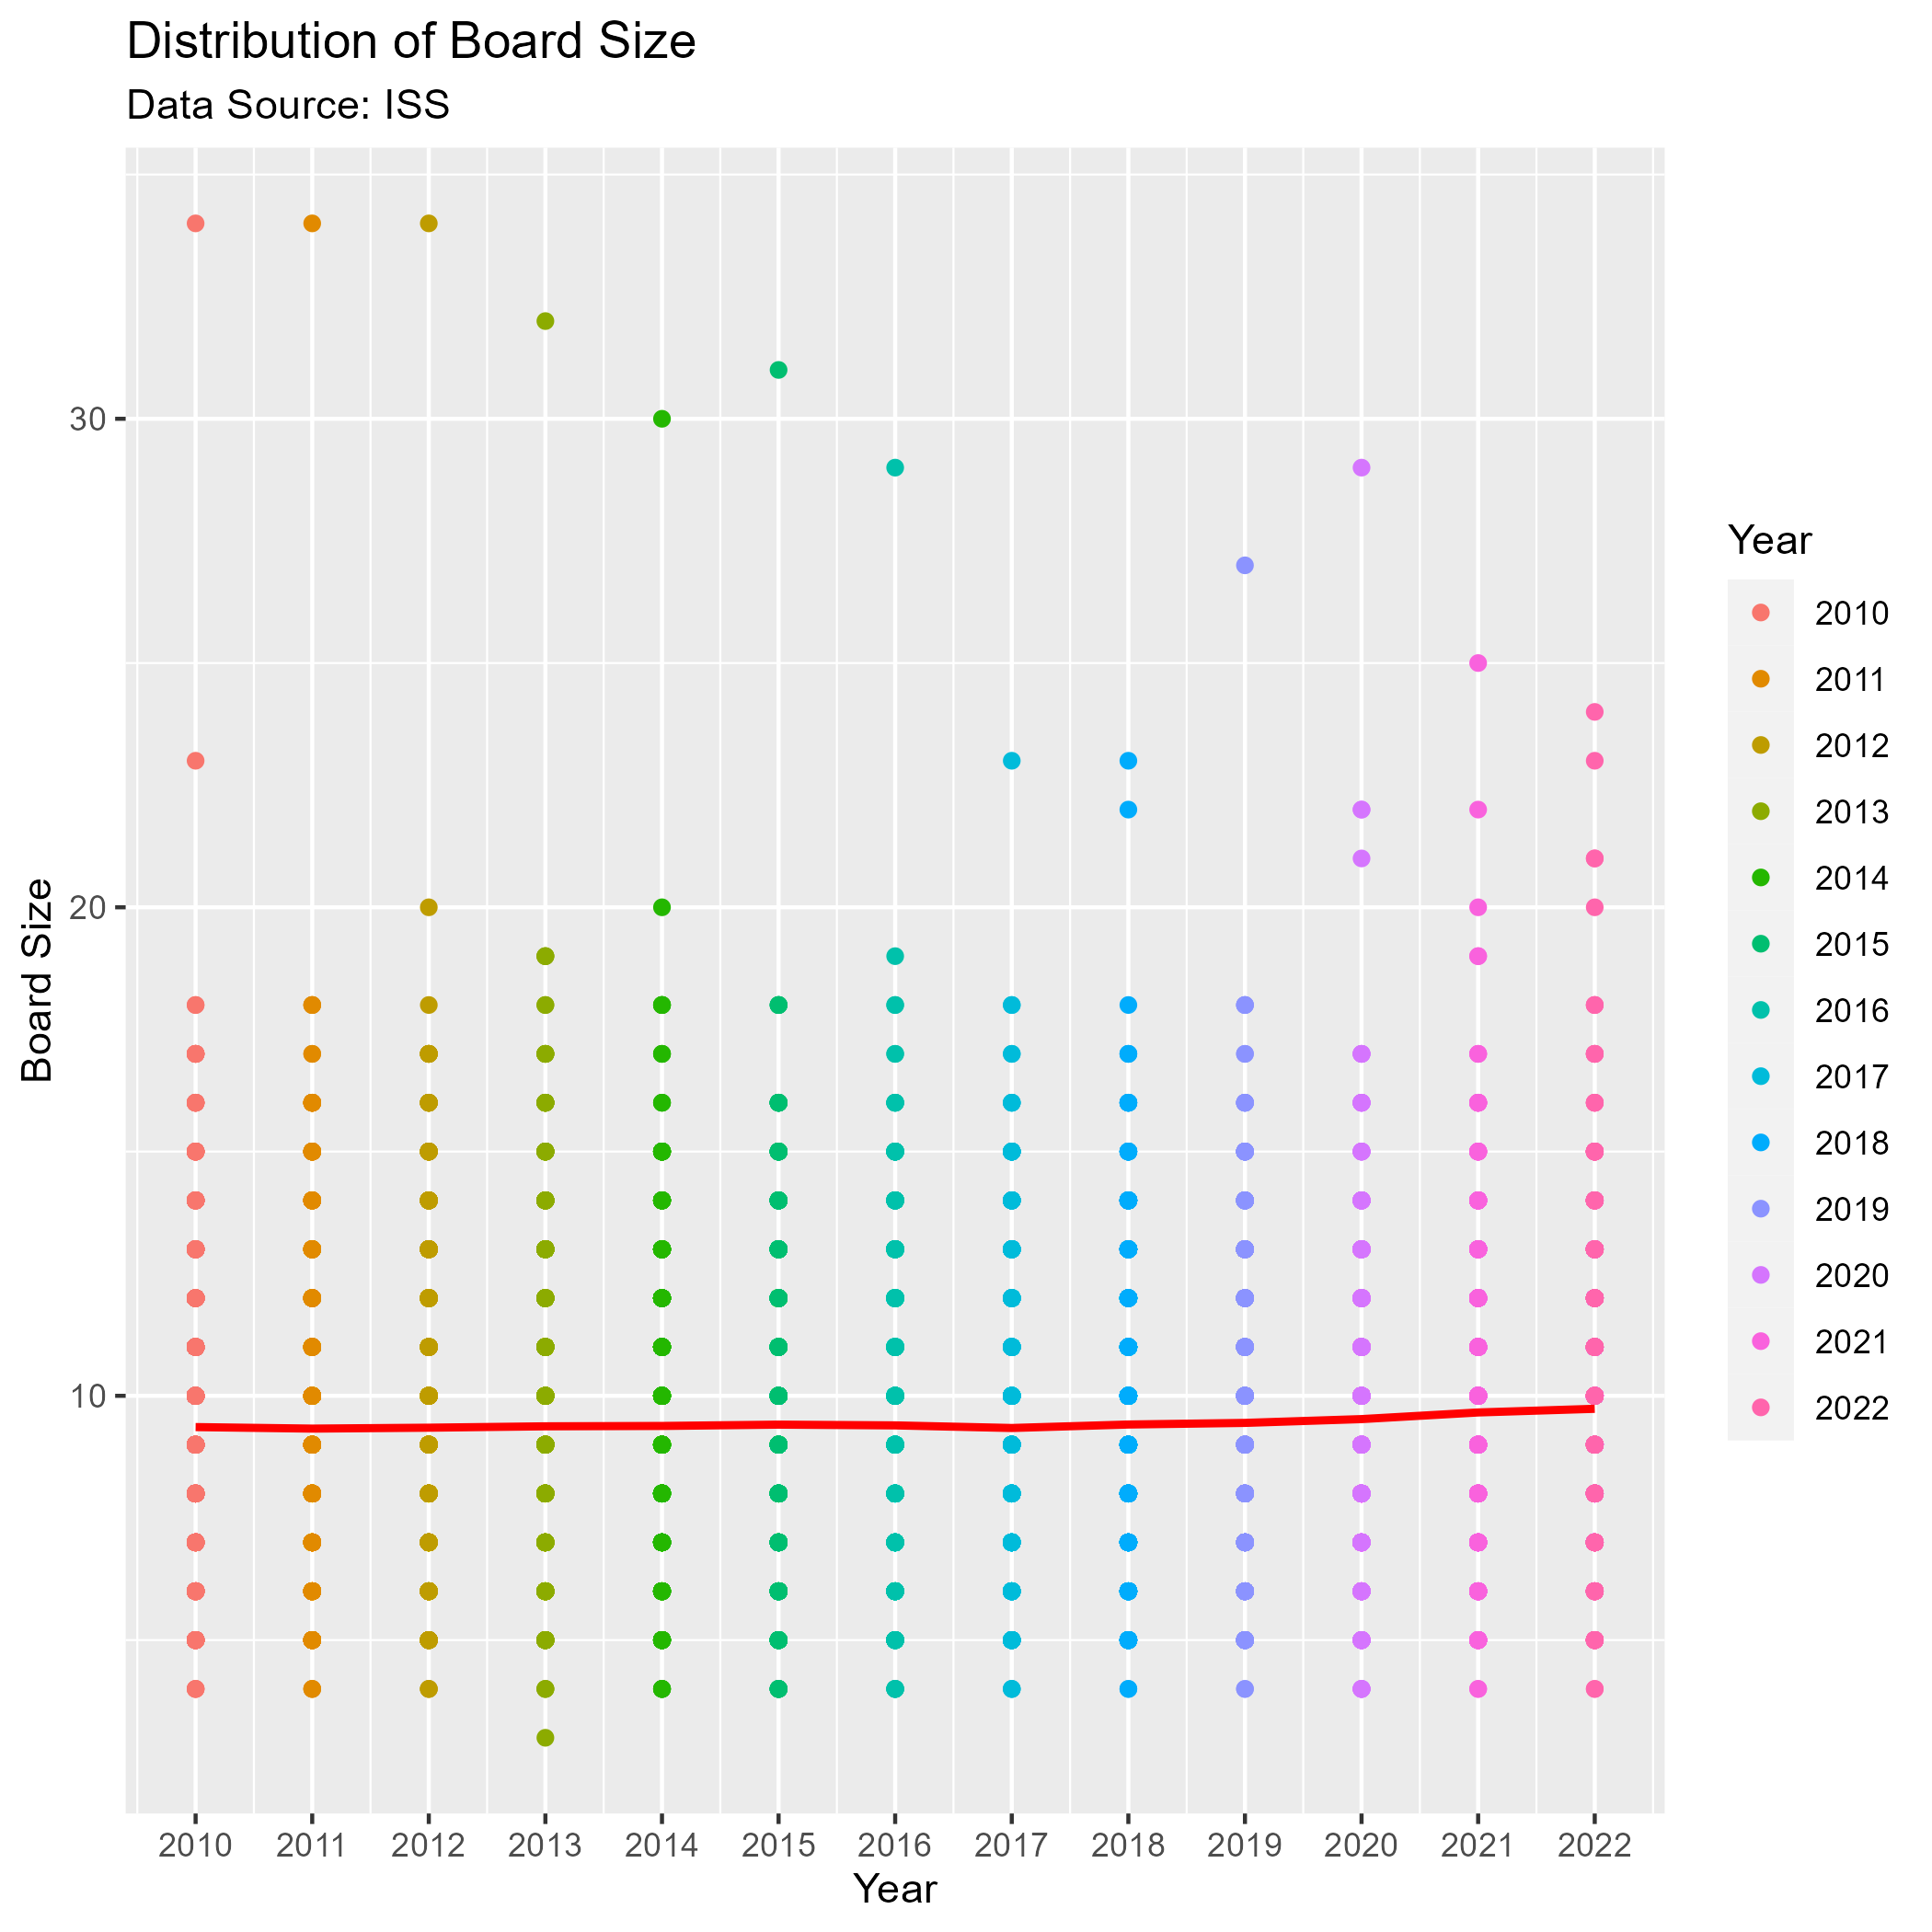
\includegraphics[width=0.4\textwidth]{PS6a_Davila.png}
  \caption{Board Size}
  \label{fig:myimage1}
\end{figure}

For the second visualization, I counted the number of distinct directors who serve on the audit committee for each firm-year to determine the audit committee size. Then, I plotted the distribution of audit committee size using a histogram. The figure below suggests that most firms have no more than 5 audit committee members, and no firm has more than 15 audit committee members. Audit committee size is a critical characteristic of public firms because it can provide valuable insights into a company's financial reporting, internal control processes, as well as its overall risk management and compliance functions.
\begin{figure}[htbp]
  \centering
  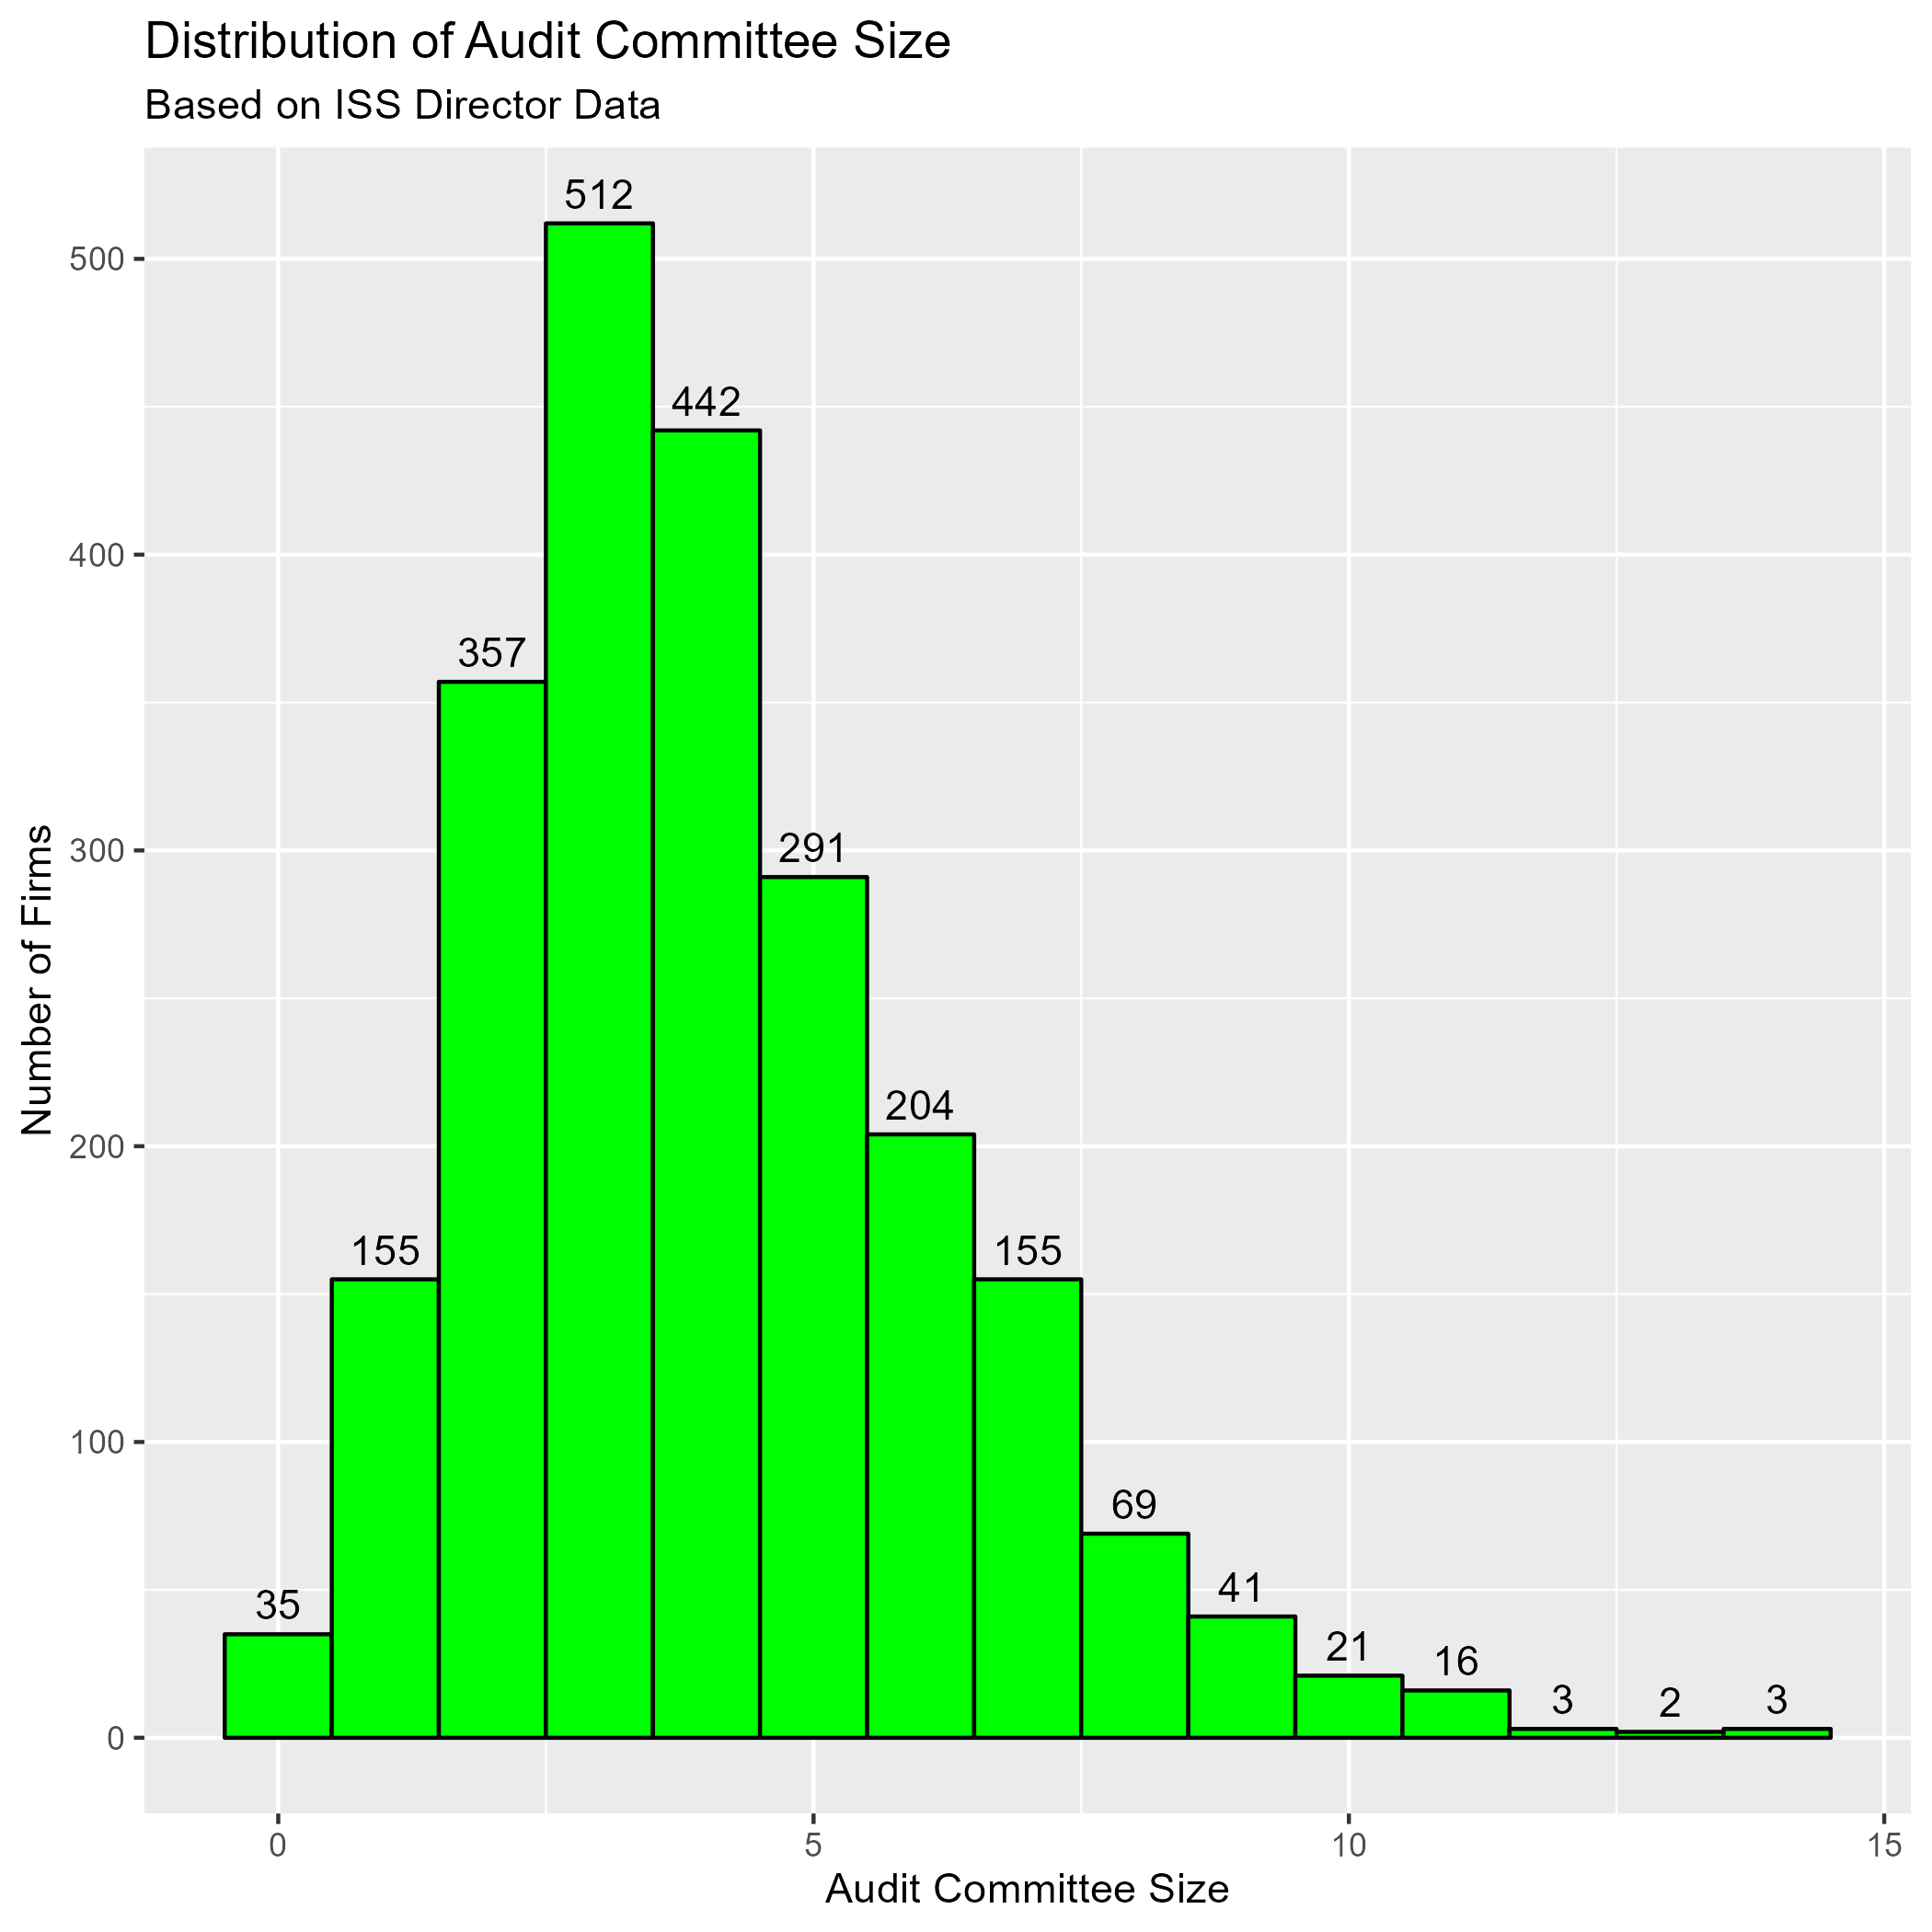
\includegraphics[width=0.4\textwidth]{PS6b_Davila.png}
  \caption{Audit Committee Size}
  \label{fig:myimage2}
\end{figure} 

For the third visualization, I counted the number of distinct independent directors for each firm and divided it by the board size to get the percentage of independent directors. Then, I created a pie chart to show the distribution of the percentage of independent directors in public firms. The figure below suggests that over half of the firms have more than 75 percent of independent directors. Independent directors are expected to provide greater transparency and accountability in the decision-making processes of the company. Thus, the percentage of independent directors is a crucial aspect of public firms' reputation and credibility.
\begin{figure}[htbp]
  \centering
  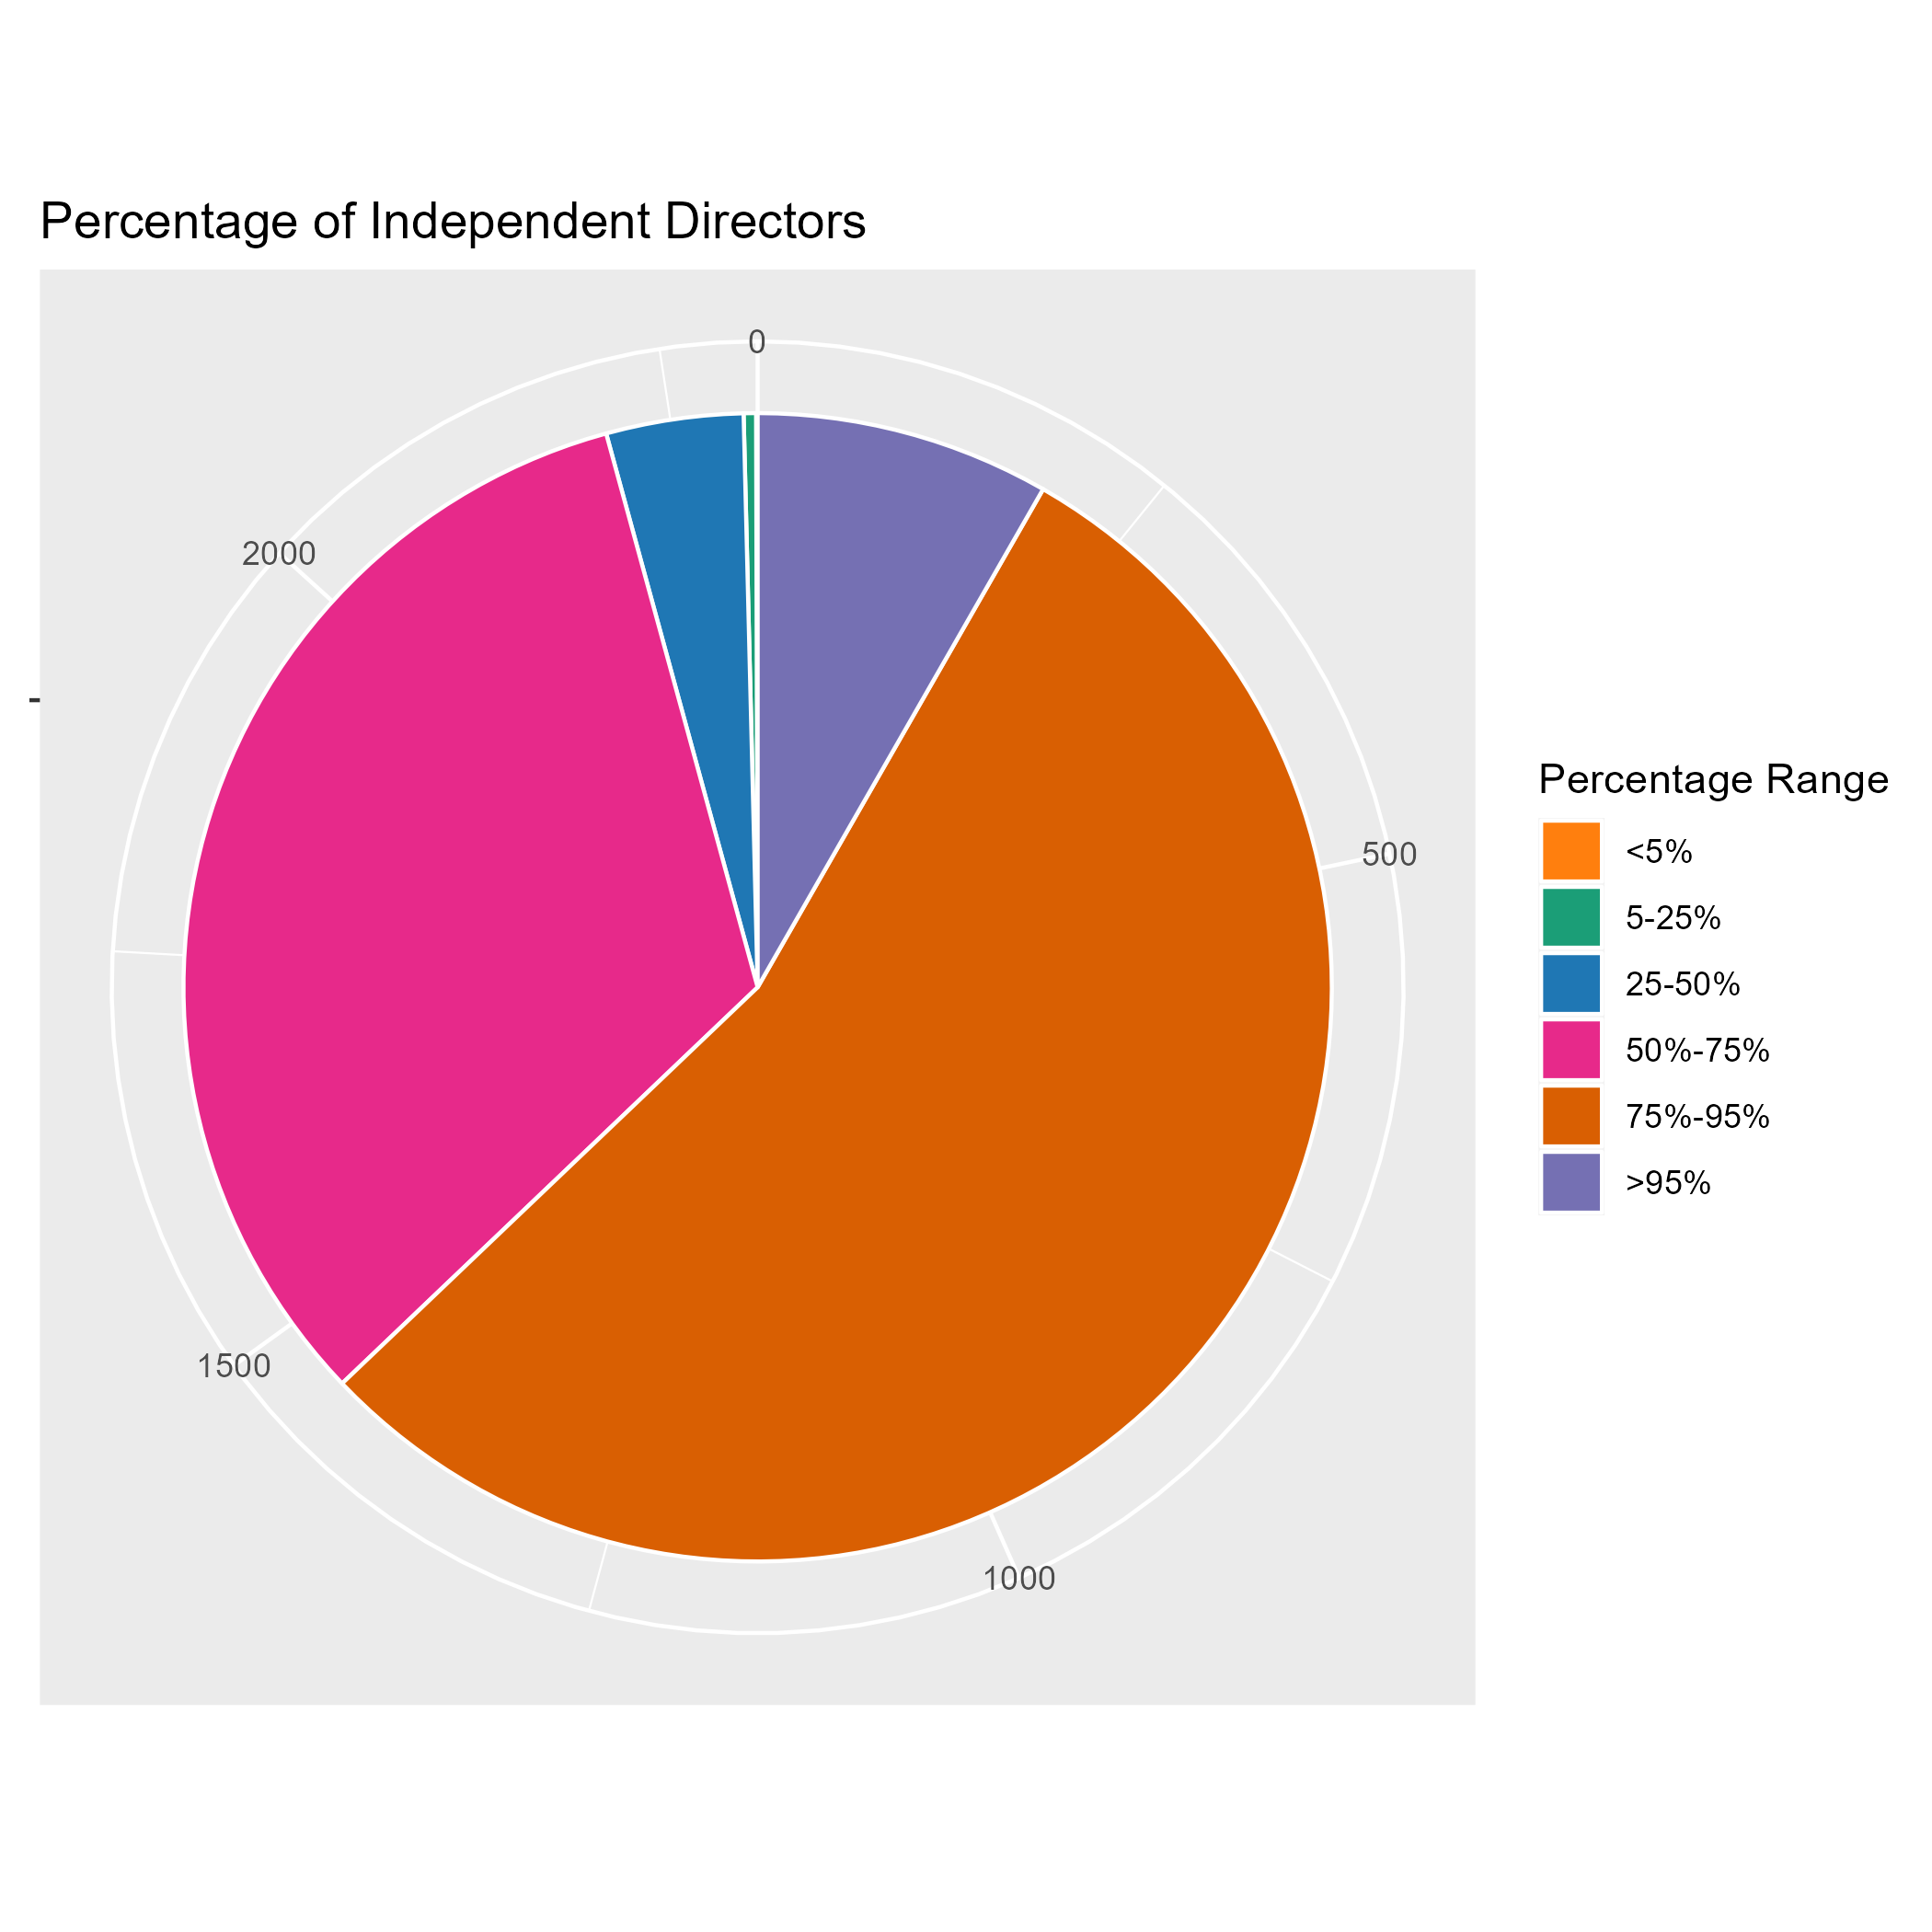
\includegraphics[width=0.4\textwidth]{PS6c_Davila.png}
  \caption{Independent Directors}
  \label{fig:myimage3}
\end{figure} 

\end{document}